\documentclass[hyperref]{ctexart}
\usepackage[left=2.50cm, right=2.50cm, top=2.50cm, bottom=2.50cm]{geometry} %页边距
\usepackage{helvet}
\usepackage{amsmath, amsfonts, amssymb} % 数学公式、符号
\usepackage[english]{babel}
\usepackage{graphicx}   % 图片
\usepackage{url}        % 超链接
\usepackage{bm}         % 加粗方程字体
\usepackage{multirow}
\usepackage{booktabs}
\usepackage{algorithm}
\usepackage{algorithmic}
\usepackage{fancyhdr} %设置页眉、页脚
\usepackage{array,tabularx}
\pagestyle{fancy}
\lhead{}
\chead{}
\lfoot{}
\cfoot{}
\rfoot{}
\usepackage{hyperref} %bookmarks
\hypersetup{colorlinks, bookmarks, unicode} %unicode
\usepackage{multicol}
\title{\textbf{正电子湮没寿命谱测量}}
\author{\sffamily 赵宇航}
\date{}
\begin{document}
\maketitle
\indent{\bf 摘要:}本实验测量了正电子湮没寿命谱,进而估算了正电子湮没的寿命并分析了其误差。\\	
\begin{multicols}{2}
\CTEXsetup[format={\Large\bfseries}]{section}
\section{实验目的}
1.了解正电子湮没寿命谱的形成原理,学会测量仪器的使用和获取正电子湮没寿命谱

2.初步掌握使用计算机解谱的数学方法和应用解谱结果来分析样品的微观结构。
	
\section{实验原理}
1928 年, Dirac 预言了正电子的存在; 1932 年, C.D.Anderson 证实了正电子的存在。近 20 年来,正电子湮没技术得到了迅猛的发展,在固体物理、金属物理和材料科学领域得到了广泛的应用。 正电子湮没技术可以分为寿命测量、 角关联测量和线形测量, 本实验进行的是寿命测量。
\subsection{正电子湮没寿命}
	从放射源发射出的高能正电子射入物质中后,首先在极短时间内(约${10}^{-12}$s以下)通过一系列非弹性碰撞减速, 损失绝大部分能量至热能, 这一过程称为注入与热化。 热化后的最后将在物质内部与电子发生湮没。 从正电子射入正电子将在样品中进行无规扩散热运动,物质到发生湮没所经历的时间一般称为正电子寿命。由于湮没是随机的, 正电子湮没寿命只能从大量湮没事件统计得出。

	在寿命测量中,最常用的正电子源是 Na-22 放射源。当它发生 β+衰变时,主要产生动能为 0-540keV 的正电子并几乎同时发射能量为 1.28MeV 的γ光子,因此,可以将此γ光子的出现作为产生正电子的时间起点, 而 0.511MeV 湮没γ 光子的出现即是正电子湮没事件的终点。这段时间间隔便可以近似地看作正电子的寿命。利用时间谱仪对每个湮没事件都可以测得湮没过程所需的时间,对足够多的湮没事件(约需 ${10}^{6}$ 次)进行记录,就得到了正电子湮没寿命谱。

	可见,所谓测量正电子湮没寿命实际上就是测量一次湮没事件中有关联的两个不同能量的 γ光子出现的时间差;将发射 1.28MeV 的 γ光子作为时间的起始信号, 而把发射 0.511MeV 的 γ光子作为终止信号。
\subsection{实验仪器}
	\begin{center}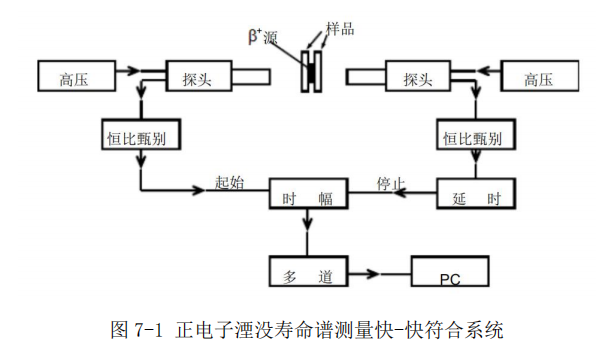
\includegraphics[scale=0.4]{t71}\end{center}
	(1)LaBr3 闪烁体探测器

	LaBr3 闪烁体探测器由 LaBr3 闪烁体及光电倍增管组成。当 γ光子射入LaBr3 闪烁体内时可发生康普顿效应,所产生的反冲电子的能量被闪烁体吸收而发生闪烁光。利用光电倍增管把微光放大并转换成电脉冲输入到相应的电子学线路中进行测量。光电倍增管由一个光阴极和多个倍增电极(通常又称为打拿极)以及阳极构成。阳极端接地,阴极端加负高压,在各打拿极上由分压电阻给出一级比一级高的电位。

	(2)数字化恒比甄别器(DCFD)

	是时间谱仪中决定时间分辨率的关键部件之一。光电倍增管输出脉冲的幅度和上升时间是随脉冲而有变化的,直接用它来触发一电子学线路时, 触发时刻会因此而出现抖动。为了解决这一问题,采用 DCFD 对光电倍增管的脉冲输出进行整理。它的作用是在每一阳极脉冲上升时间的一恒定点上产生一信号,使输入到时间幅度转换器的脉冲起始 (或终止) 时间与光电倍增管脉冲输出的起始时间之间有一恒定的时间差,不受光电倍增管输出脉冲幅度等变化的影响,而只决定于光子γ发射的时刻。这就显著地提高了测量的准确度。

	(3)时幅转换器

	将 DCFD 输出的起始信号与另一个 DCFD 输出的终止信号之间的时间差线性地转换为一脉冲的幅度。其测量原理如下:时间分析器相当于一个恒流源在电流开关 K 的控制下对电容 C 充电;起始信号使开关 K 接通,而终止信号使 K断开。

	根据电学基本知识,电容 C 上的电压幅度 V 与充电时间 t 的关系为下式表明,由于 I 和 C 都是恒定的,输出脉冲的幅度正比于两个信号的时间差。
	\begin{equation}
	V_C=\frac Q C=\frac{I}{C}t
	\end{equation}

	由于时幅转换器本身有一定的 “死时间”;当小于此时间时, 不能得到线性转换。 因此,为了保证时间差信号都能得到线性转换, 终止信号在输入到时间幅度转换器前先通过一延时器,其延迟时间可以按需要进行调节。 由时间分析器输出的信号可直接送入微机多道分析器(接在 ADC IN 上),由后者经过模数转换后时间差存贮在相应道址的存贮器中。利用延时器还能对时间谱仪进行时间标定.

	(4)数字多道分析器

	将输入脉冲按不同幅度分类计数, 即不同幅度的脉冲计入不同的道址中。在多道分析器中道址与时间或能量 (在本实验中为时间) 相对应作为横坐标,而每道中的计数 (即记录到的一定寿命的湮没事件的发生次数)作为纵坐标。这样就可以得到一个正电子湮没寿命谱。

\section{实验结果}
	\subsection{实验数据绘图}
	以下分别对应【Start 能窗选择】和【Stop能窗选择】选择 (1.28MeV , 0.511MeV),(0.511MeV , 1.28MeV),(0.511MeV , 0.511MeV) ,(1.28MeV , 1.28MeV) 
	\begin{center}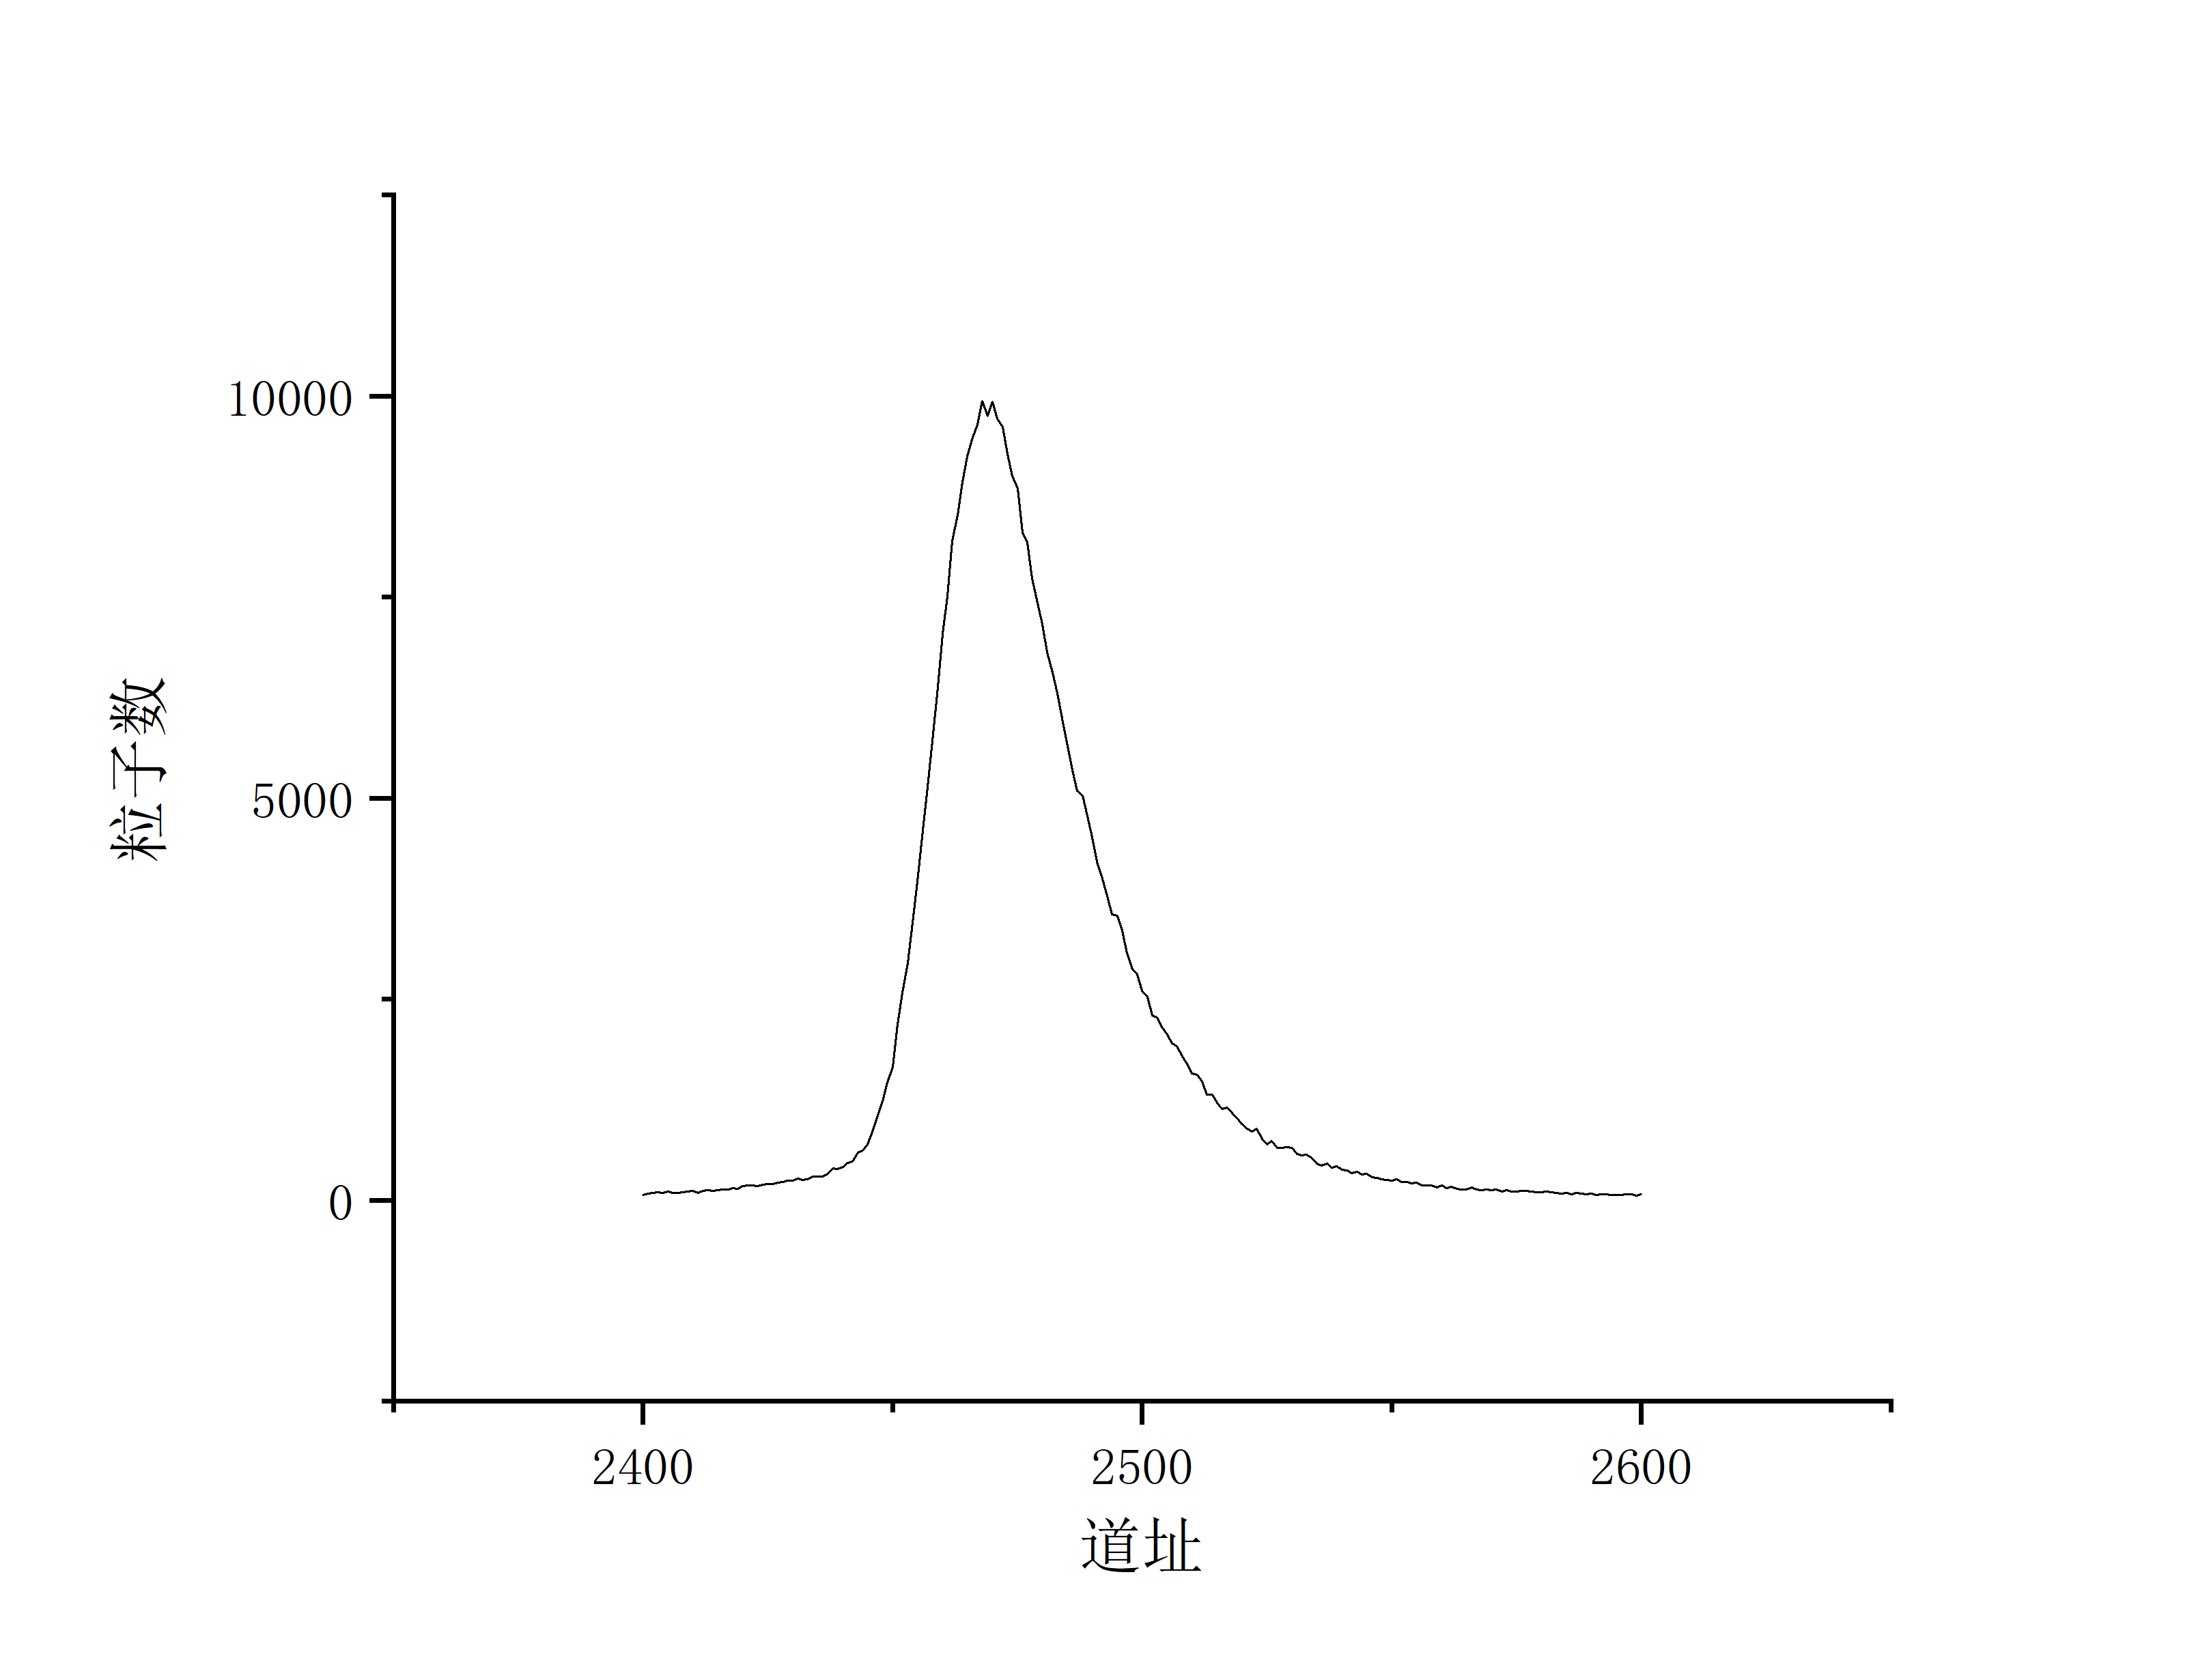
\includegraphics[scale=0.3]{t11.png}\end{center}
	\begin{center}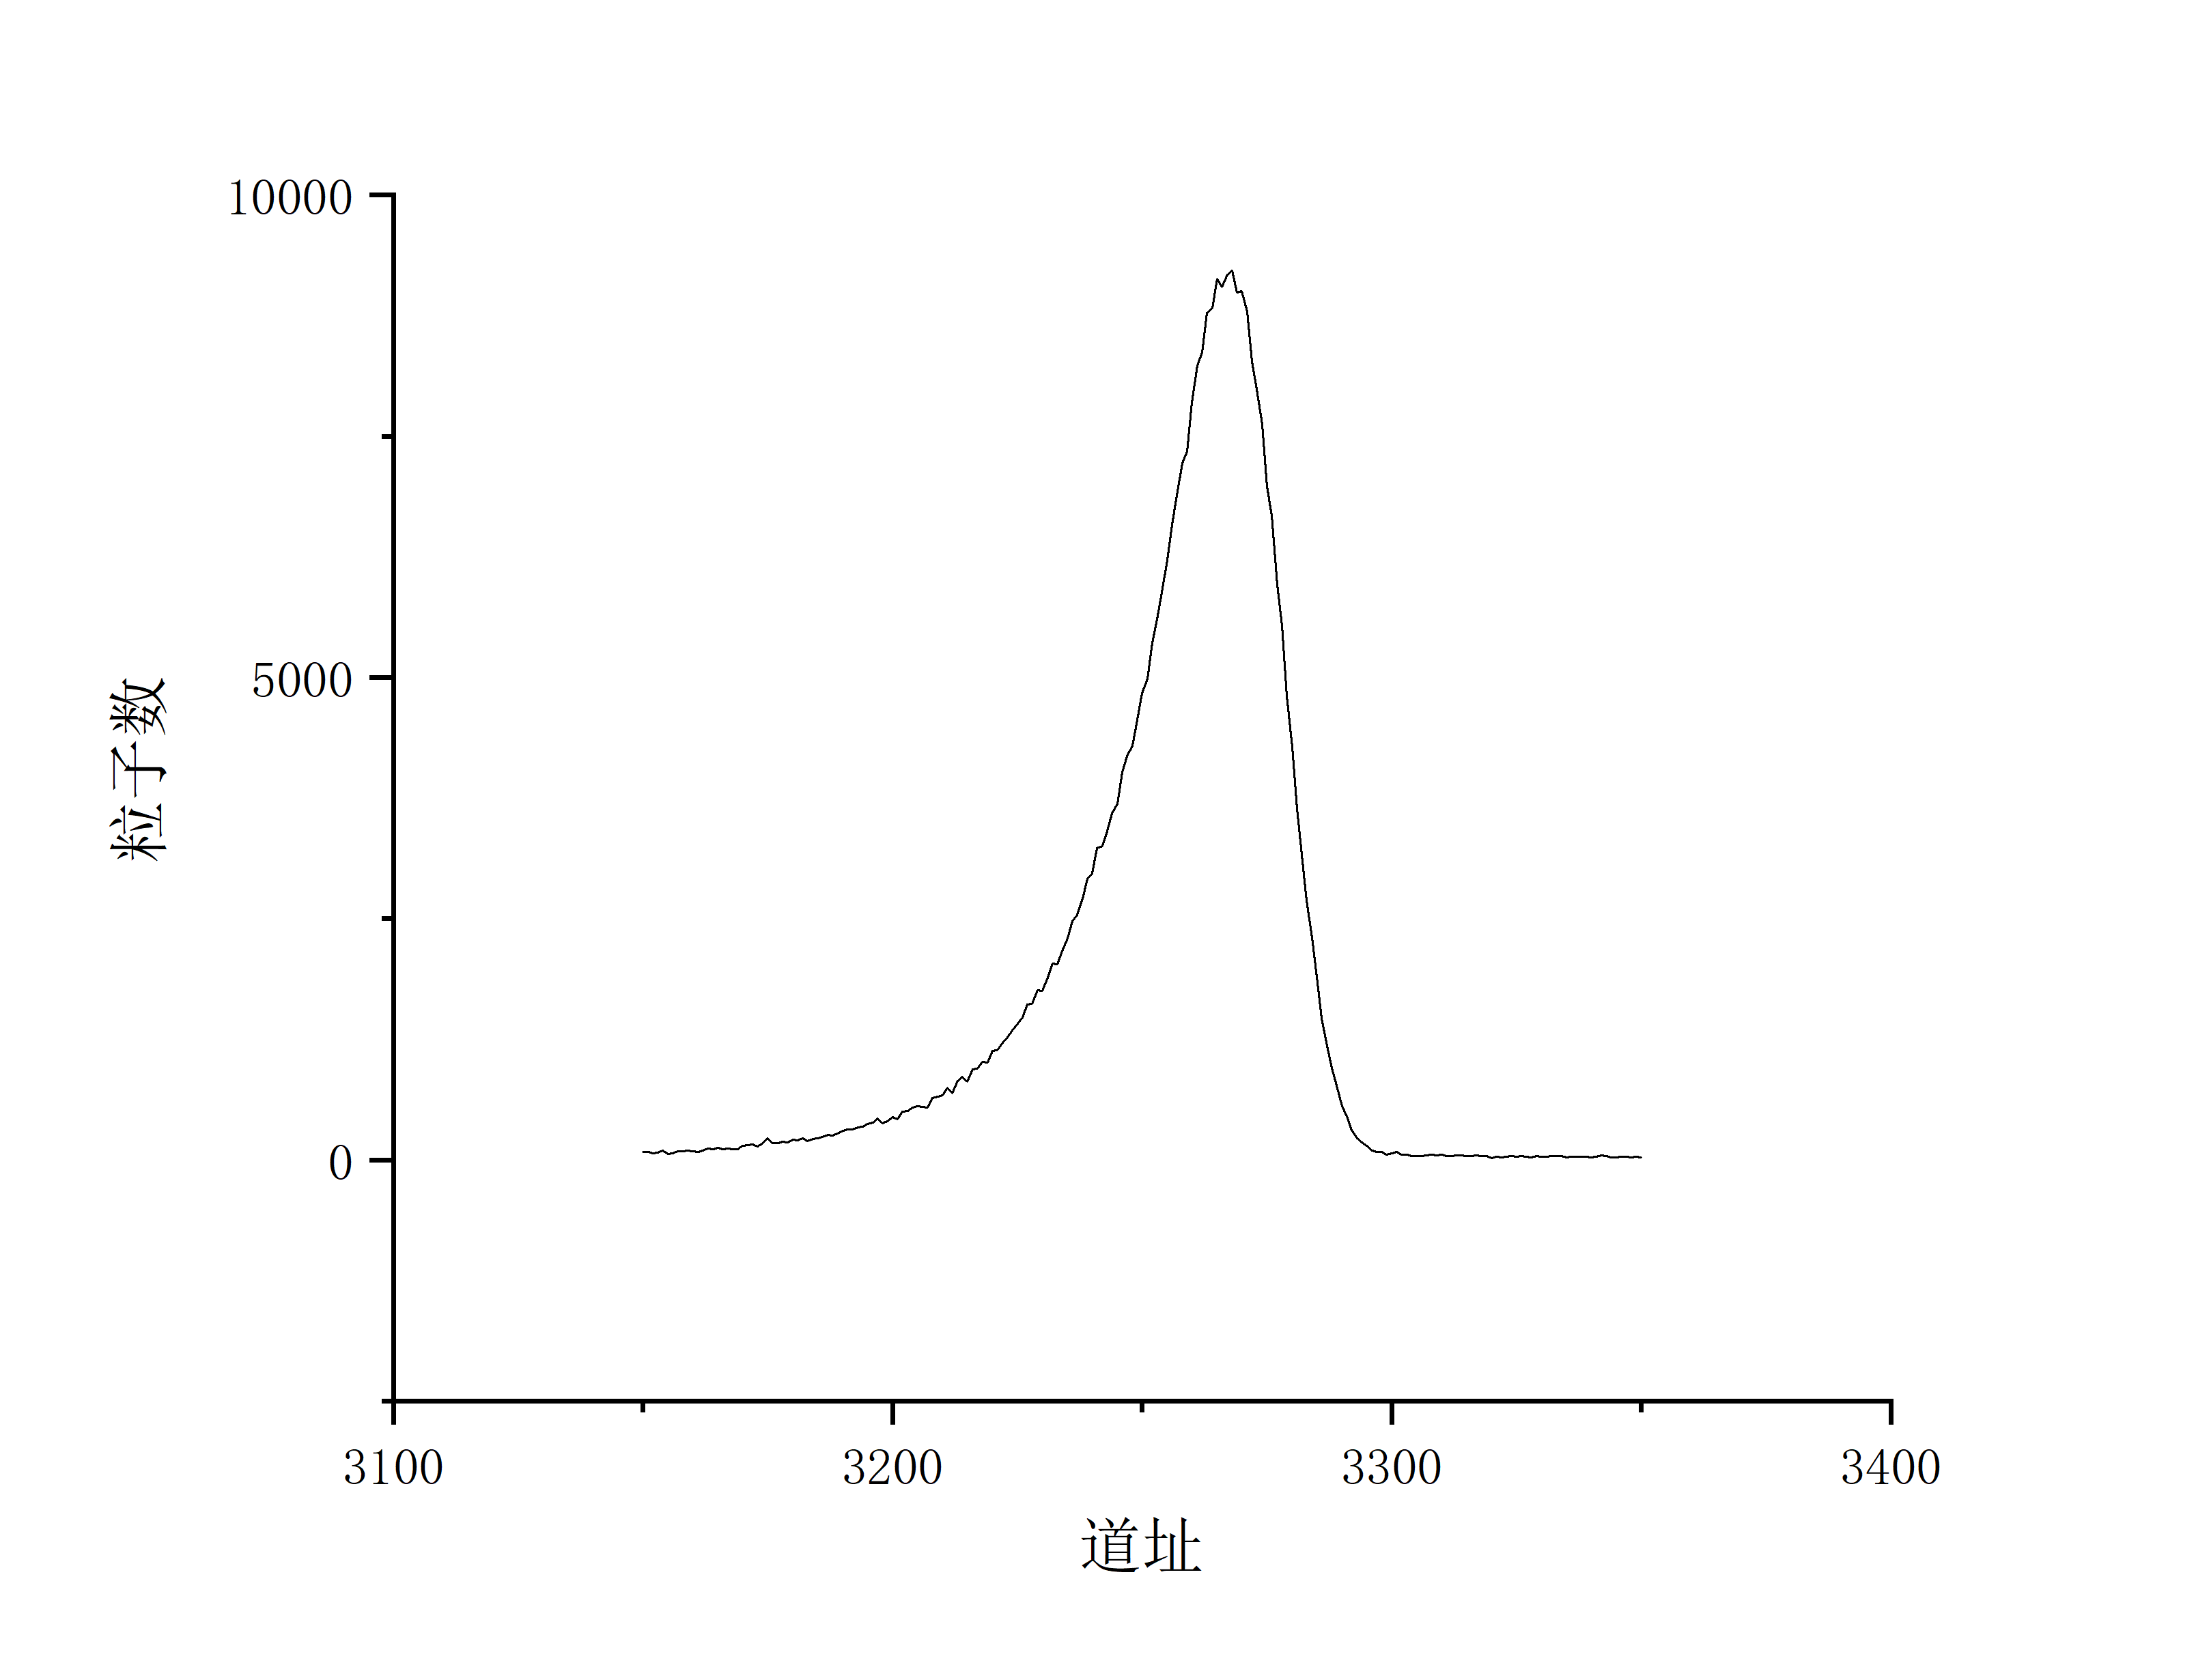
\includegraphics[scale=0.3]{t12.png}\end{center}
	\begin{center}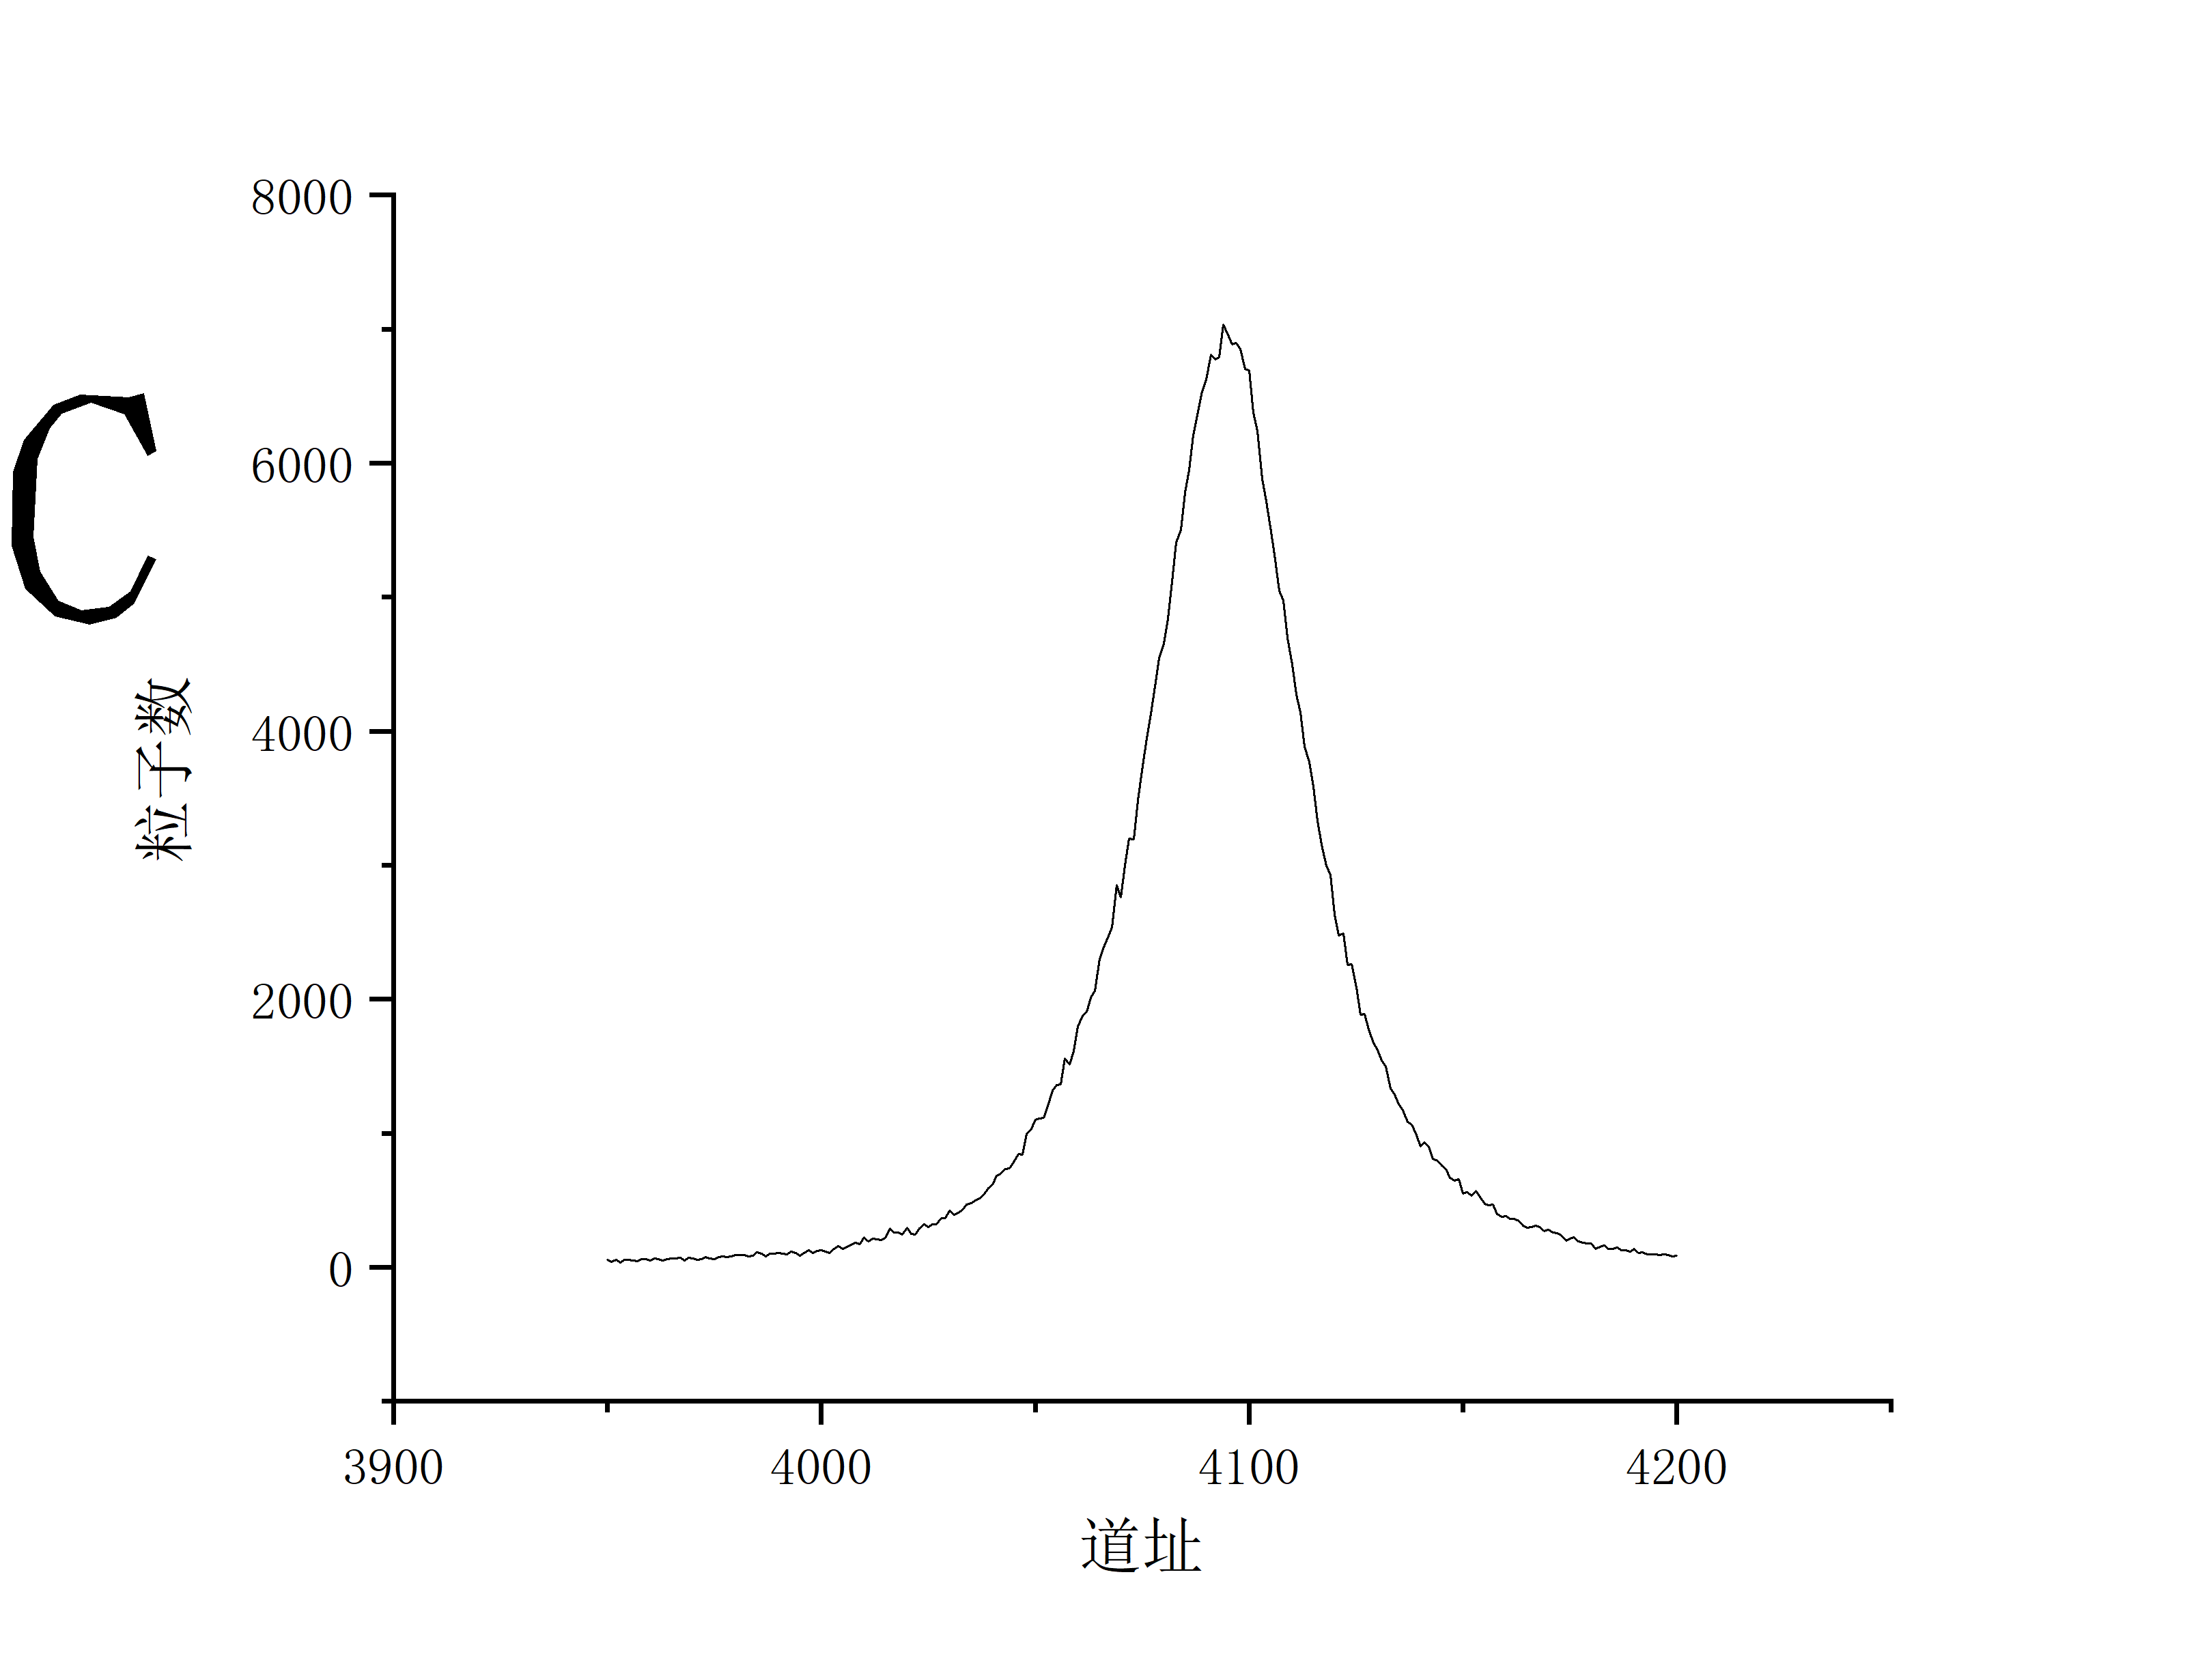
\includegraphics[scale=0.3]{t13.png}\end{center}
	\begin{center}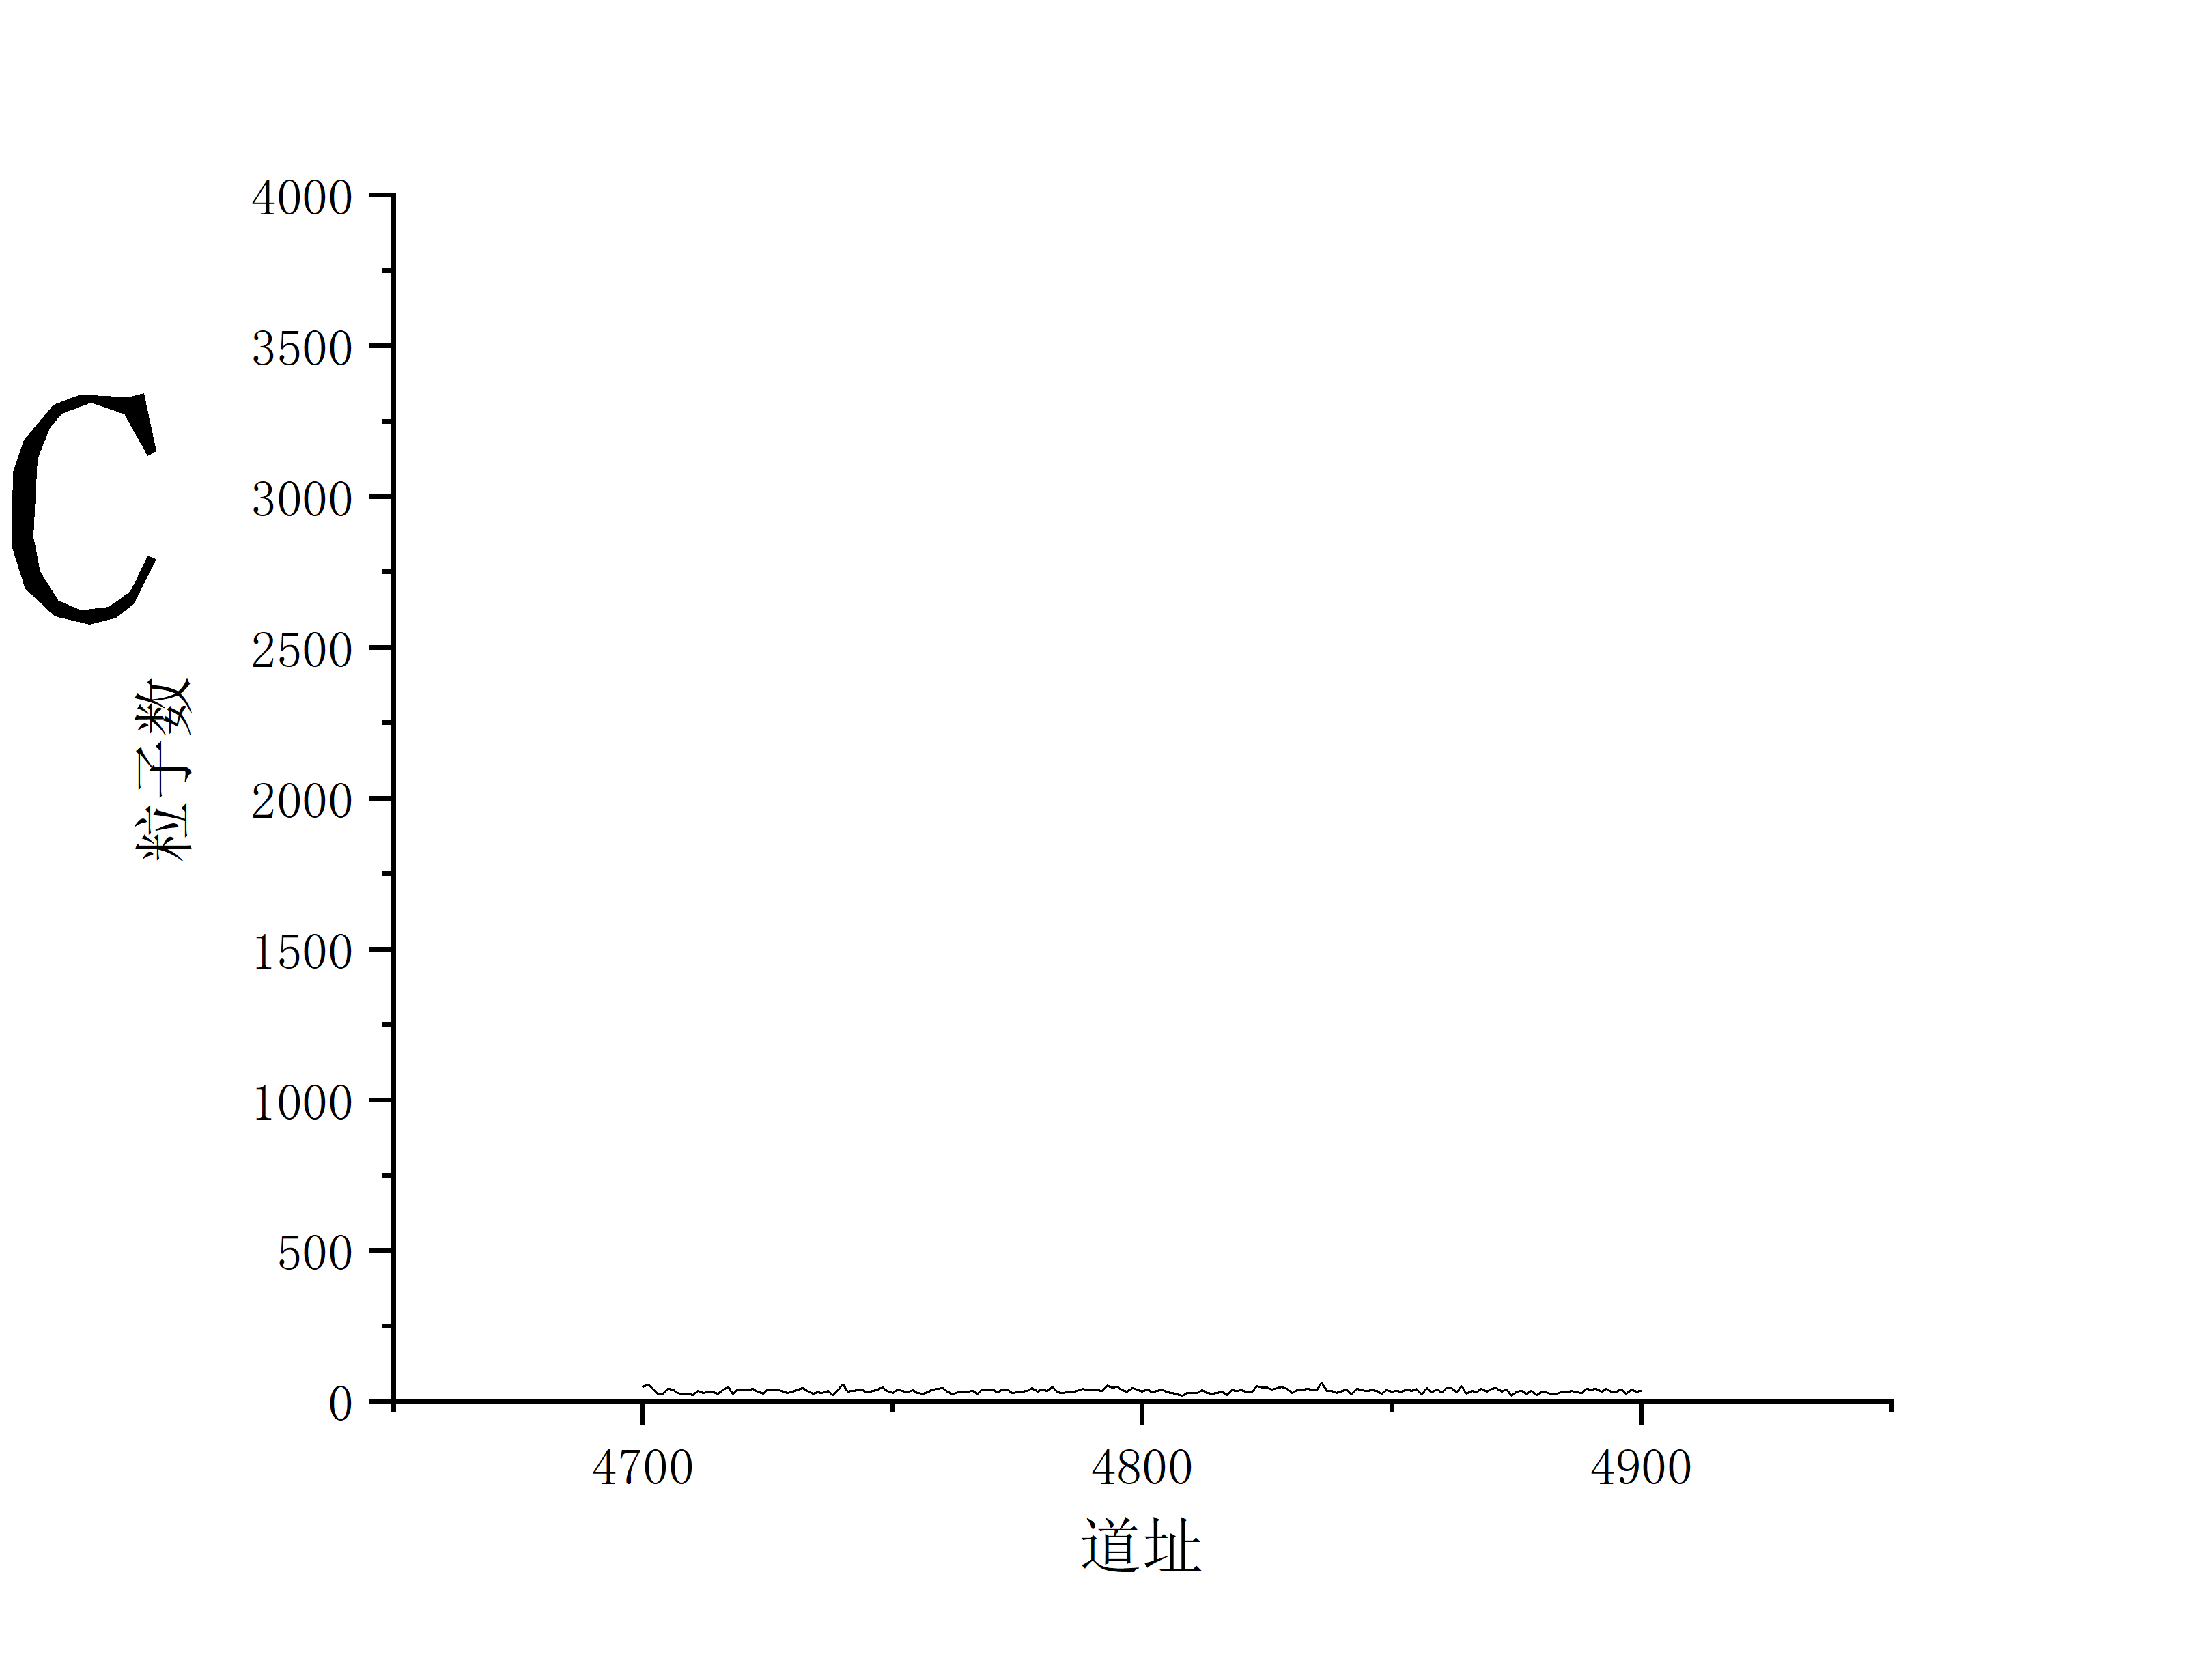
\includegraphics[scale=0.3]{t14.png}\end{center}

	寿命谱实际上测的是两特定谱线的时间差,选择不同的起止能窗,时间差一般认为不同,所以寿命谱不同。

	\subsection{寿命成分计算}
	根据20ns延迟所得峰位道址1650.08 ,30ns延迟所得峰位道址2469.23 ,可以得到增益大约为$819 /ns$。取道址1-1000可以算得环境样底大约为$32 $。剔除环境影响后,取30ns延迟的实验数据直接加权求得正电子湮没寿命约为$0.26ns $。

	我们把数据按道址等距分为三份,考虑到等效负寿命,前两份作为一份与后一份等同。然后将这两份作为两组寿命组成成分(这里实际上是需要软件解谱,限于条件我们手动模拟这个过程)。

	在之前的计算中,我们取总计数373157 ,注意到此时正电子湮没寿命为0.26272ns 。选取寿命组成成分之后,第一份粒子数358362 ,占比$96.0\%$,计算得寿命约为0.23937ns 。第二份粒子数14795 ,占比$4.0\%$,计算得寿命约为1.1227ns 。如下表
	$$\begin{tabular}{|c|c|c|}
	\hline
	{} & 第一成分 & 第二成分  \\ \hline
	寿命 & 0.2397ns & 1.1227ns  \\ \hline
	强度 & 96.0\% & 4.0\%  \\ \hline
	\end{tabular}$$

依次求得第一份方差为0.0237 ,第二份方差为0.0452 。将第一份相邻道址粒子数取均值,考虑到第一份粒子数远大于第二份,以第一份粒子数为基准权重,求得两份协方差为0.0225 。协方差矩阵如下
	$$\left( \begin{matrix}
	0.0237 & 0.0225 \\
	0.0225 & 0.0452
	\end{matrix}\right)$$
	
可以求得相关系数0.687 。

	\subsection{与标准样品比较}
	查资料得,金属中正电子自由态湮没的典型寿命值为170ps 。我们所测得时间为263ps 。如果要分析实验样品的微观结构变异情况,我们考虑0.511MeV谱线的出现。事实说明,它延后了。有可能是样品比较稀疏,正电子进入样品后未能及时与负电子相遇。
\section{讨论}
	Na-22 放射源强度太弱,测量效率低,需要等很久才有足够多的计数降低误差;容易与环境混淆,对甄别器精度要求高。Na-22 放射源强度太强会损伤样品。

	恒比甄别器会判断光子能量并进行筛选,如果设置在相应能窗的下阈以上,那么对应的能量就会与环境噪声一同被过滤,不能通过甄别器。从而不被记录失掉湮没事件。




\end{multicols}
\end{document}